\documentclass{article}
\usepackage[utf8]{inputenc}
\usepackage[english]{babel}
\usepackage[]{amsthm}
\usepackage[]{amssymb}
\usepackage[]{amsmath}
\usepackage[]{graphicx}
\usepackage[]{hyperref}
\usepackage[]{xcolor}
\usepackage[]{cancel}
\usepackage[]{fancyhdr}
\hypersetup{
    colorlinks,
    linkcolor={red!50!black},
    citecolor={blue!50!black},
    urlcolor={blue!80!black}
}

\pagestyle{fancy}
\fancyhf{}
\title{\vspace{-4cm}MTH20012 - Series and Transformations Test 2}
\author{Joshua Rogers}
\lhead{MTH20012 Test 2}
\rhead{Joshua Rogers 101096819}
\date\today

\begin{document}
\maketitle 

\section*{Part B Question 5}

\[ f(t) = \begin{cases} 
      4 & 0\leq t < 6 \\
      -\frac{5}{6}t+9 & 6\leq t < 12
   \end{cases}
\]

\subsection*{A}

We let $u=t$ and $dv=cos(at)$, thus $du = 1$ and $v = \frac{sin(at)}{a}$
\begin{align*}
\int t cos(at) dt =&\\
&\frac{tsin(at)}{a} - \int \frac{sin(at)}{a} dt\\
= &\frac{tsin(at)}{a} + \frac{cos(at)}{a^2}
\end{align*}

\subsection*{B}

We let $u=t$ and $dv=sin(at)$, thus $du = 1$ and $v = -\frac{cos(at)}{a}$
\begin{align*}
\int t sin(at) dt =&\\
&-\frac{tcos(at)}{a} - \int -\frac{cos(at)}{a} dt\\
= &-\frac{tcos(at)}{a} + \frac{sin(at)}{a^2}
\end{align*}

\subsection*{C}
See image below.
\begin{figure}
\centering
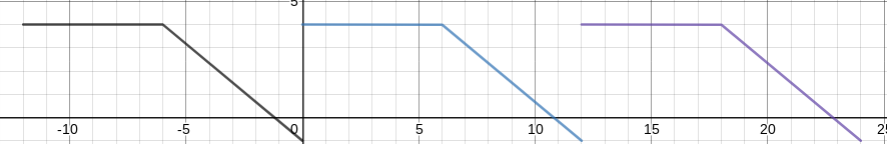
\includegraphics[width=1.0\textwidth]{./static/graph3.png}
\caption{Part C}
\end{figure}


\end{document}
